57. $\cfrac{4}{x^2-x-6}\geqslant\cfrac{1}{2+x}\Leftrightarrow\cfrac{4}{(x-3)(x+2)}-\cfrac{1}{x+2}\geqslant0\Leftrightarrow
\cfrac{7-x}{(x-3)(x+2)}\geqslant0.$ Применив метод интервалов, найдём ответ:
\begin{figure}[ht!]
\center{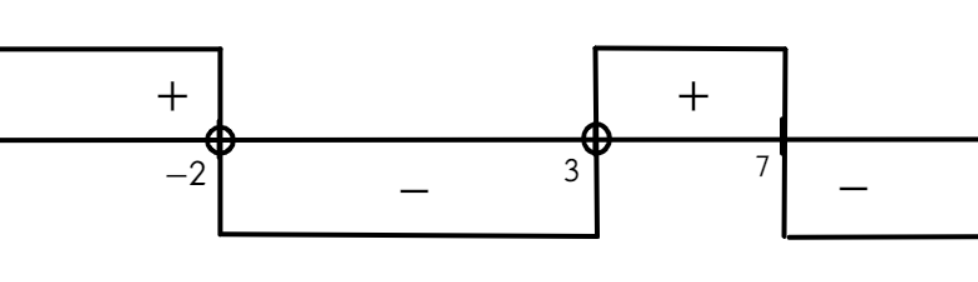
\includegraphics[scale=0.35]{int57.png}}
\end{figure}
$x\in(-\infty;-2)\cup(3;7].$\\
